\input{mmd-article-header}
\def\mytitle{BOSH Tutorial}
\def\myauthor{VMware 2012 - Cloud Foundry}
\def\latexmode{memoir}
\input{mmd-article-begin-doc}
\chapter{Introduction}
\label{introduction}

This tutorial will guide you through the process of deploying a multi-tier WordPress installation using BOSH. Due to its simplicity, WordPress is a good way to learn BOSH, but it is not meant to represent a realistic use case.

\chapter{Prerequisites}
\label{prerequisites}

A working BOSH director

\chapter{Installing BOSH on an Ubuntu VM}
\label{installingboshonanubuntuvm}

\section{Install Ruby via rbenv}
\label{installrubyviarbenv}

\begin{enumerate}
\item BOSH is written in Ruby. Let's install Ruby's dependencies

\begin{verbatim}
sudo apt-get install git-core build-essential libsqlite3-dev curl libmysqlclient-dev libxml2-dev libxslt-dev libpq-dev
\end{verbatim}


\item Get the latest version of rbenv

\begin{verbatim}
cd
git clone git://github.com/sstephenson/rbenv.git .rbenv
\end{verbatim}


\item Add \texttt{\ensuremath{\sim}\slash .rbenv\slash bin} to your \texttt{\$PATH} for access to the \texttt{rbenv} command-line utility

\begin{verbatim}
echo 'export PATH="$HOME/.rbenv/bin:$PATH"' >> ~/.bash_profile
\end{verbatim}


\item Add rbenv init to your shell to enable shims and autocompletion

\begin{verbatim}
echo 'eval "$(rbenv init -)"' >> ~/.bash_profile
\end{verbatim}


\item Download Ruby 1.9.2

\begin{verbatim}
wget http://ftp.ruby-lang.org/pub/ruby/1.9/ruby-1.9.2-p290.tar.gz
\end{verbatim}


\item Unpack and install Ruby

\begin{verbatim}
 tar xvfz ruby-1.9.2-p290.tar.gz
 cd ruby-1.9.2-p290
 ./configure --prefix=$HOME/.rbenv/versions/1.9.2-p290
 make
 make install
\end{verbatim}


\item Restart your shell so the path changes take effect

\begin{verbatim}
source ~/.bash_profile
\end{verbatim}


\item Set your default Ruby to be version 1.9.2

\begin{verbatim}
rbenv global 1.9.2-p290
\end{verbatim}


\end{enumerate}

\section{Install Local BOSH and BOSH Releases}
\label{installlocalboshandboshreleases}

\begin{enumerate}
\item Sign up for an account on the Cloud Foundry public Gerrit server at \href{http://reviews.cloudfoundry.org/}{http:/\slash reviews.cloudfoundry.org\slash }\footnote{\href{http://reviews.cloudfoundry.org/}{http:/\slash reviews.cloudfoundry.org\slash }}

\item Generate an ssh public key (accept all defaults)

\begin{verbatim}
ssh-keygen -t rsa
\end{verbatim}


\item Copy your key from \texttt{\ensuremath{\sim}\slash .ssh\slash id\_rsa.pub} into your Gerrit account

\item Set your name and email

\begin{verbatim}
        git config --global user.name "Firstname Lastname"
        git config --global user.email "your_email@youremail.com"
\end{verbatim}


\item Install our gerrit-cli gem:

\begin{verbatim}
        gem install gerrit-cli
        rbenv rehash
\end{verbatim}


\item Clone BOSH repositories from Gerrit

\begin{verbatim}
        gerrit clone ssh://[<your username>@]reviews.cloudfoundry.org:29418/bosh-sample-release.git
        gerrit clone ssh://[<your username>@]reviews.cloudfoundry.org:29418/release.git
        gerrit clone ssh://[<your username>@]reviews.cloudfoundry.org:29418/bosh.git
\end{verbatim}


\item Run some rake tasks to install the BOSH CLI

\begin{verbatim}
cd ~/bosh
rake bundle_install (Note: if this fails run 'gem pristine rake' and retry)
cd cli
bundle exec rake build
gem install pkg/bosh_cli-x.x.x.gem
\end{verbatim}


\end{enumerate}

\section{Deploy to your BOSH Environment}
\label{deploytoyourboshenvironment}

With a fully configured environment, we can begin deploying the sample application to our environment. As listed in the prerequisites, you should already have an environment running, as well as the IP address of the BOSH Director. Ask your BOSH technical contact for help if you need it.

\subsection{Point BOSH at a Target and Clean your Environment}
\label{pointboshatatargetandcleanyourenvironment}

\begin{enumerate}
\item Target your director (this IP is an example - replace with yours!) 

\begin{verbatim}
bosh target 192.168.1.99:25555 
\end{verbatim}


\item Check the state of your BOSH settings.

\begin{verbatim}
bosh status
\end{verbatim}


\item The result of your status will be akin to:

\begin{verbatim}
Target         targetname (http://198.1621.99:25555) Ver: 0.3.12 (01169817)
UUID           #####hex-uuid-goes-here-############
User           admin
Deployment     not set
\end{verbatim}


\item If you have previously used this BOSH director you may have existing deployments and releases. List previous deployments (we will remove them in a moment)

\begin{verbatim}
bosh deployments
\end{verbatim}


\item If you have any existing deployments \texttt{bosh deployments} will show something like:

\begin{verbatim}
+---------+
| Name    |
+---------+
| example |
+---------+
\end{verbatim}


\item Delete any existing deployments (ex: example) 

\begin{verbatim}
bosh delete deployment example 
\end{verbatim}


\item Answer \texttt{yes} to the prompt and wait for the deletion to complete

\item List previous releases (we will remove them in a moment)

\begin{verbatim}
`bosh releases`
\end{verbatim}


\item If you have result of \texttt{bosh releases} should be akin to:

\begin{verbatim}
+--------+----------+
| Name   | Versions |
+--------+----------+
| myapp  | 1, 2, 3  |
+--------+----------+
\end{verbatim}


\item Delete the existing releases (ex: myapps) 

\begin{verbatim}
bosh delete release myapp 
\end{verbatim}


\item Answer \texttt{yes} to the prompt and wait for the deletion to complete

\end{enumerate}

\subsection{Create a Release}
\label{createarelease}

\begin{enumerate}
\item Change directories into bosh-sample-release:

\begin{verbatim}
cd ~/bosh-sample-release
\end{verbatim}


This directory contains the sample WordPress deployment and release files. 

\item Reset your environment

\begin{verbatim}
bosh reset release
\end{verbatim}


\item Answer \texttt{yes} to the prompt and wait for the environment to be reset

\item Create a release

\begin{verbatim}
bosh create release --force --with-tarball
\end{verbatim}


\item Answer \texttt{wordpress} to the \texttt{release name} prompt

\item Your terminal will display information about the release including the Release Manifest, Packages, Jobs, and tarball location.

\item Open \texttt{bosh-sample-release\slash wordpress.yml} in your favorite text editor and confirm that \texttt{name} is \texttt{wordpress} and \texttt{version} matches the version that was displayed in your terminal (if this is your first release, this will be version 1).

\end{enumerate}

\subsection{Deploy the Release}
\label{deploytherelease}

\begin{enumerate}
\item Upload the WordPress example Release to your Environment

\begin{verbatim}
bosh upload release dev_releases/wordpress-1.tgz
\end{verbatim}


\item Your terminal will display information about the upload, and an upload progress bar will reach 100\% after a few minutes.

\item Open \texttt{bosh-sample-release\slash wordpress.yml}. You will need to edit several things to match your environment. You should update director\_uuid, any VLANs, the IPs under networks, dns servers and any static ips listed for specific jobs. An example manifest is in the Appendix.

\item Deploy the Release

\begin{verbatim}
bosh deploy
\end{verbatim}


\item Your deployment will take a few minutes.

\item Copy the URL for your WordPress installation from the \texttt{properties.wordpress.servername} value in \texttt{wordpress.yml}

\item Browse your WordPress blog at this URL.

\item Complete the form to install your WordPress blog

\end{enumerate}

\begin{figure}[htbp]
\centering
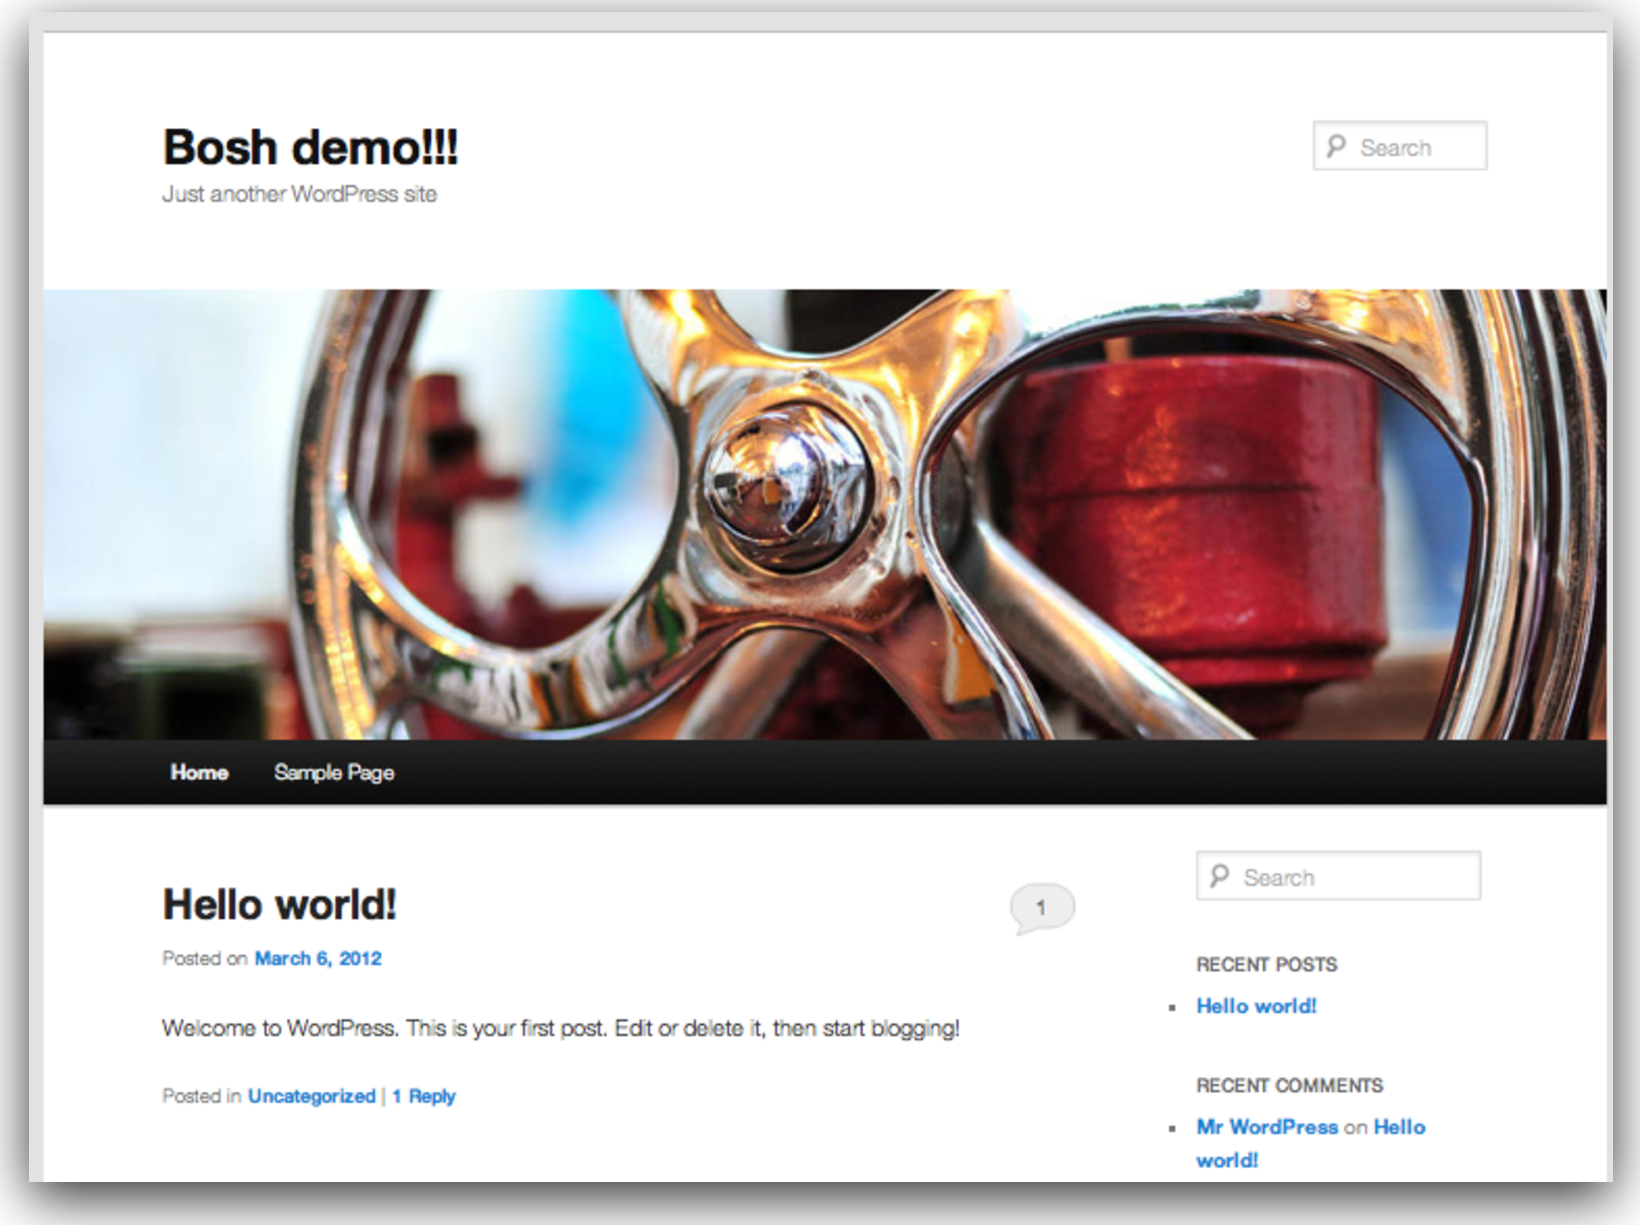
\includegraphics[keepaspectratio,width=\textwidth,height=0.75\textheight]{deployed.pdf}
\caption{Deployed Wordpress}
\label{}
\end{figure}



\section{Appendix}
\label{appendix}

\begin{adjustwidth}{2.5em}{2.5em}
\begin{verbatim}

    ---
    name: wordpress
    director_uuid: #####hex-uuid-goes-here-############

    release:
        name: wordpress
        version: 1

    compilation:
        workers: 4
        network: default
        cloud_properties:
            ram: 2048
            disk: 8096
            cpu: 2

    # this section describes how updates are handled

    update:
        canaries: 1
        canary_watch_time: 30000
        update_watch_time: 30000
        max_in_flight: 4
        max_errors: 1

    networks:
    - name: default
        subnets:
        - reserved:
            - 192.168.224.2 - 192.168.224.10
            - 192.168.224.200 - 192.168.224.254
        static:
            - 192.168.224.11 - 192.168.224.100
            range: 192.168.224.0/23
            gateway: 192.168.224.1
        dns:
            - 192.168.1.4
            - 192.168.1.5
        cloud_properties:
            name: VLAN1234

    - name: dmz
      subnets:
      - static:
        - 192.168.4.241 - 192.168.4.242
      range: 192.168.4.241/28
      dns:
            - 192.168.1.4
            - 192.168.1.5
        cloud_properties:
      cloud_properties:
        name: VLAN4321

    resource_pools:

        - name: infrastructure
        network: default
        size: 6
        stemcell:
            name: bosh-stemcell
            version: 0.4.7
        cloud_properties:
            cpu: 1
            disk: 8192
            ram: 4096

    jobs:
        - name: mysql
        template: mysql
        instances: 1
        resource_pool: infrastructure
        persistent_disk: 16384
        networks:
            - name: default
            static_ips:
                - 192.168.224.11

        - name: wordpress
        template: wordpress
        instances: 4
        resource_pool: infrastructure
        networks:
            - name: default
            static_ips:
                - 192.168.224.12 - 192.168.224.15

        - name: nginx
        template: nginx
        instances: 1
        resource_pool: infrastructure
        networks:
            - name: default
                default: [dns, gateway]
                static_ips:
                    - 192.168.224.1
            - name: dmz
                static_ips:
                    - 192.168.4.241

    properties:
        wordpress:
            admin: foo@bar.com
            port: 8008
            servers:
                    - 192.168.224.12
                    - 192.168.224.13
                    - 192.168.224.14
                    - 192.168.224.15
            servername: wp.myurl.mycompany.com
            db:
                name: wp
                user: wordpress
                pass: w0rdpr3ss
            auth_key: random key
            secure_auth_key: random key
            logged_in_key: random key
            nonce_key: random key
            auth_salt: random key
            secure_auth_salt: random key
            logged_in_salt: random key
            nonce_salt: random key
        mysql:
            address: 192.168.224.11
            port: 3306
            password: verysecretpasswordforroot
        nginx:
            workers: 1

\end{verbatim}
\end{adjustwidth}

\input{mmd-memoir-footer}

\end{document}
